\newpage
\section{Problem description}
The Android application that we used for gathering our data set is an application that supports users using public transport. Given the current location it will provide you with an up-to-date timetable of the next buses and trains that depart from your closest stations as well as when they leave and where they're going. It uses data freely available from the SBB Open Data Initiative. \cite{SBBOpenData} 

The application contains an opt-in service that allows gathering usage data of the application. When a user has opted-in and is using the application, this service will gather information about the closest station and the timestamp and send it to a server where it is permanently stored. The data also includes an anonymized user id to identify the data points to the specific user. This is the data set that we worked with for our thesis. Each entry includes the user id, the station id and the timestamp of when the data point was collected. The reference data didn't contain any structure otherwise, so we started out with a flat file including the full data set. The data set and the analysis we've done on it are described in further detail in section~\ref{subsec:data_set}. We have enhanced each raw data point with the previous station the user was at as well as the next station he went to. The next station is what will be used as ground truth in our predictions.

Due to the way the data is gathered in the application and the fact that in a single trip the application will store a data point for each station that is passed (with its respective timestamp) we can conclude that our data points are dependant on each other. An individual data point should not be looked at in isolation because the meaning of the gathered data point can change for our prediction. To successfully predict the next station we need to have information in our historical data about the movements between the stations and not just the stations themselves. Therefore we have modeled our problem as a sequence prediction problem. Sequence prediction is discussed in more detail in the following section. 

\subsection{Sequence Prediction}
As machine learning is a very broad field covering lots of different use cases and is based on differing assumptions it is crucial to first analyze the kind of problem that is being tackled by applying machine learning techniques. Without a fond and thorough understanding of the domain and the available data it's nearly impossible to get a useful result and conclusion from experimenting. Just as it is a lot harder for a normal human being to deduce useful information and to learn something given some random, unstructured, unprepared, redundant or even wrong data it is also not possible (at least not yet) for a computer (i.e. a machine learning algorithm) to make sense of such a heap of data. Data needs to be analyzed, prepared, structured and combined before being fed to the algorithm in order to fully unveil its usefulness. If we do not properly prepare the data and find patterns, we are almost certain to run into indescribable issues or results later on in the process. \cite{DataMining} 

Many machine learning algorithms are created for independent, identically distributed data.\cite{MachineLearningTUMunich} They work under the assumptions that two data points should not correlate and have no explicit influence on each other. In our thesis this is not the case. We explicitly combine data from different data points (such as what was the last station before this one). Therefore we have modeled our problem as a sequence prediction, or sequence learning problem.

Sequence prediction deals with sequential data. A machine learning algorithm that allows for sequential data should not make the assumption that data points are independent, should account for distortion and should also use contextual information whenever available. Popular use cases for algorithms using sequence prediction are time-series predictions (e.g. weather forecasting, stock market predictions, geographical tracking predictions) and sequence labeling (e.g. speech recognition, handwriting recognition, gesture recognition). There are different types of algorithms that fall under this technique, such as different supervised learning classifiers (e.g. Decision Trees, Probabilistic Algorithms, Support Vector Machines, Neural Networks). In our experiments we have included several different algorithms from the field of sequence prediction.

\subsection{Proposed Solutions}
\label{subsec:proposed_solution}
We used multiple different techniques to solve our task and to use in the final evaluation. A decision tree algorithm, a naive Bayes algorithm as well as a multilayer perceptron algorithm (which falls under the Neural Networks category). The theoretical foundation of these algorithms are described here in further detail. The practical way in which we used them are described in Section~\ref{subsec:machine_learning_results}. As a machine learning toolkit we have used WEKA.

\subsubsection{WEKA}
\label{subsection:WEKA}
In order to not need to reinvent the wheel when it comes to implementing the actual algorithms we have built our solution on top of WEKA, the machine learning toolkit provided by the University of Waikato, New Zealand. WEKA is a collection of machine learning algorithms as well as tools for data processing, clustering, classification, visualization and more. It can also be used to develop new machine learning schemes. WEKA is written in Java and can be used by any JVM-based programming language. Its algorithms can be directly used on a dataset. We only used a subset of the features provided by WEKA. We didn't use any of the visualization tools. Since we also did all the preprocessing and analysis ourselves we didn't need any of the features WEKA provides in that part. What we were interested in is the implementation of the classifiers as well as the actual training, testing and evaluation of the classifiers. As is described later in this thesis we used the provided implementations of the classifiers we propose. 

\subsubsection{Decision Trees}
Decision tree learning in the context of data mining is a technique using a decision tree as a predictive model to map observations about input data. These observations help come to a conclusion about the data's target value. A tree model that accepts a finite set of values is called a "classification tree", in case continuous values are allowed the decision tree is called "regression tree". A decision tree doesn't explicitly represent a decision, however the resulting classification tree can be used as an input for decision making. 

In a decision tree model, a leaf represents a class label and a branch represents a conjunction of features leading to the class labels. As can be seen in the example in Figure \ref{fig:image-decision-tree} the interior nodes correspond to the input values, the edges are the value domain and the leafs represent the values of the target variable. With such a modeled decision tree we can easily either visually or computationally evaluate new input data and derive the target values.

\begin{figure}[!ht]
	\centering
		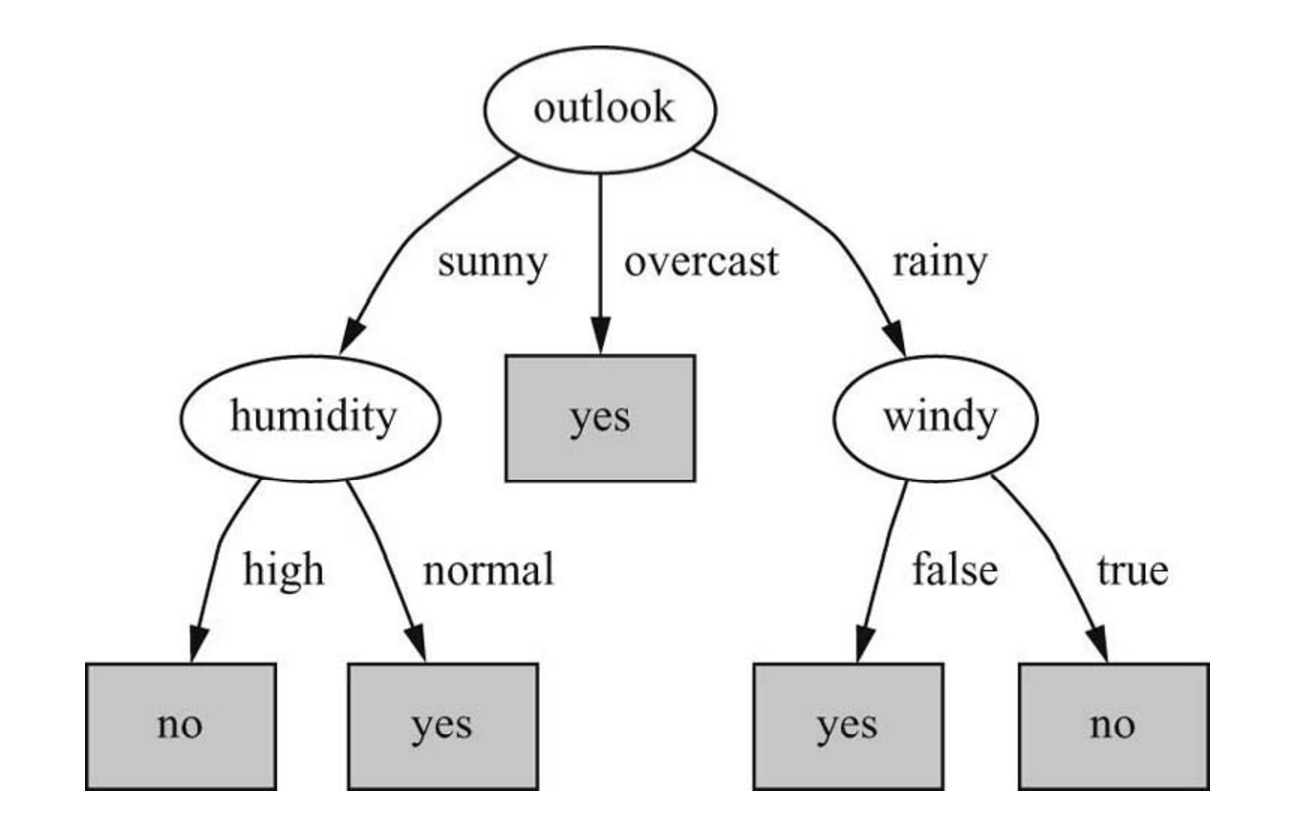
\includegraphics[width=1.0\textwidth]{images/decision-tree}
	\caption{An example of a decision tree \cite{WikipediaDecisionTrees}}
	\label{fig:image-decision-tree}
\end{figure}

A tree can be trained or learned by splitting the source data set into subsets based on testing the attribute values. In order to get the full model of the decision tree, this process has to be repeated until a subset at a node has only one value or until splitting no longer adds value to the predictions. This process is called recursive partitioning and is the most common strategy to train decision trees.

There are many variants to a simple decision tree that use a combination of multiple decision trees. Examples algorithms are Random Forests, Rotation Forests or Bagging Decision Trees. In addition there are different algorithms that implement decision trees. They usually focus on a different metric that they want to optimize. 

Decision Trees have many advantages. They are quite simple to understand and reason about. They also require relatively little data preparation. An additional advantage is that necessary computing resources are quite low, even when using large datasets.


\subsubsection{Naive Bayes}
Naive Bayes classifiers are simple probabilistic classifiers that are based on Bayes theorem, assuming independence of features. On an abstract level, given a vector representing some features, the naive Bayes will assign a probability to all possible outcomes (also called classes) given this vector. It is a condition probability model. Based on Bayes' theorem, a reliable and computable model can be constructed for all the possibilities that need to be generated. From the naive Bayes probability model we can then construct a classifier. The naive Bayes classifier usually combines the probability model with a decision rule. This rule will define, which hypothesis is to be picked. A common rule is to simply pick the one with the highest probability, which is also called "maximum a posteriori" (MAP) decision rule.

Advantages of naive Bayes classifiers are also their simplicity. If the conditional independence assumptions of the feature are fully given, it will also converge faster than other models. One of the disadvantages that come with conditional independence is that it won't be able to model relations between features properly. 


\subsubsection{Multilayer Perceptron (Neural Network)}
A multilayer perceptron is a special case of an artificial neural network. Artificial neural networks work on a simplified model of how the human brains work. They generate layers of nodes, each having certain input and output values. The nodes (also called neurons) are triggered by an activation function. This function can can take many shapes and be triggered by a combination or a series of inputs of a neuron. Once the activation function has triggered, the neuron will send its output signal throughout the outgoing channels. This might then trigger the next row of activation functions in the next layer of the network, until the output of the network is reached. An example graph of a multilayer perceptron (as a neural network) is shown in figure \ref{fig:multilayer-perceptron}.

\begin{figure}[!ht]
	\centering
	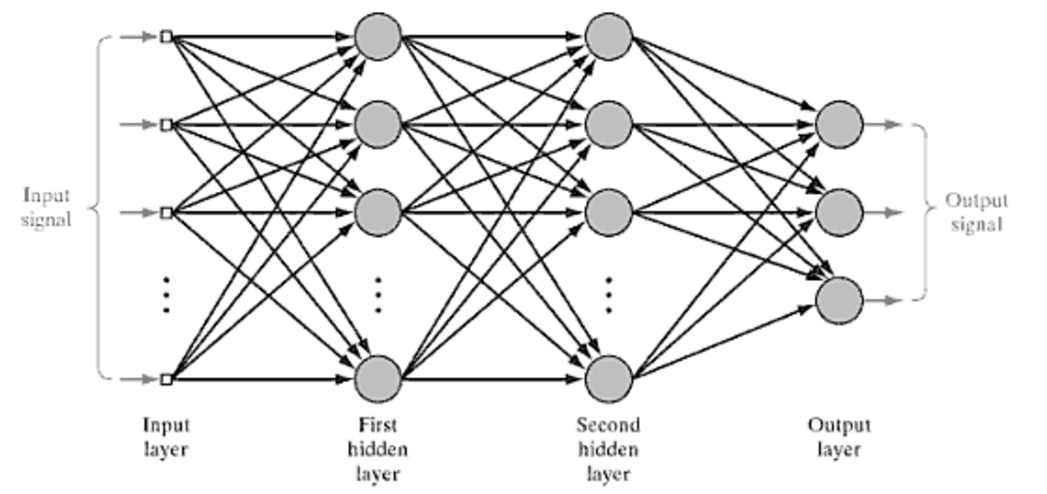
\includegraphics[width=1.0\textwidth]{images/multilayer-perceptron}
	\caption{An example of a multilayer perceptron \cite{MultilayerPerceptron}}
	\label{fig:multilayer-perceptron}
\end{figure}

A multilayer perceptron consists of multiple layers in a forward directed graph, each layer connected only to the next one. Every neuron in the layer has a non-linear activating function to properly model the way neurons in the biological brain are activated. A multilayer perceptron has at least three layers, an input, output and one or more hidden layers. Since it always includes at least one hidden layer it is considered a deep neural network.

A multilayer perceptron is trained using backpropagation. In the beginning of the training stage all weights of all neurons are set to a default value. Based on the errors in the output of each of the training data entry the weights of the neurons are adapted. Once the network is in a stable state and the weights don't change anymore the training can be considered to be completed.